\laborator{Лабораторная работа моделирование теплообменных процессов}

\goal составить математическую модель теплообменников с различной структурой потоков.

\subsubsection{Теория}
Практически ни одно производство, а в химической технологии тем более, не обходится без процессов которые необходимо проводить при определенной температуре. Процесс теплообмена может рассматриваться индивидуально (в случае теплообменников), или в совокупности с процессами массопередачи и химическими реакциями.

В зависимости от организации подвода или отвода тепла структура потока теплоносителей может описываться различными моделями. В связи с тем, что модель идеального вытеснения имеет наибольшую движущую силу, в промышленности наиболее распространение получили аппараты наиболее близкие к данной структуре потока: кожухотрубчатые, <<труба в трубе>>, пластинчатые и другие. На рисунке  \ref{fig:heat.scheme1} представлена схема потоков в прямоточном теплообменнике.

\begin{figure}[h]
	\begin{center}
		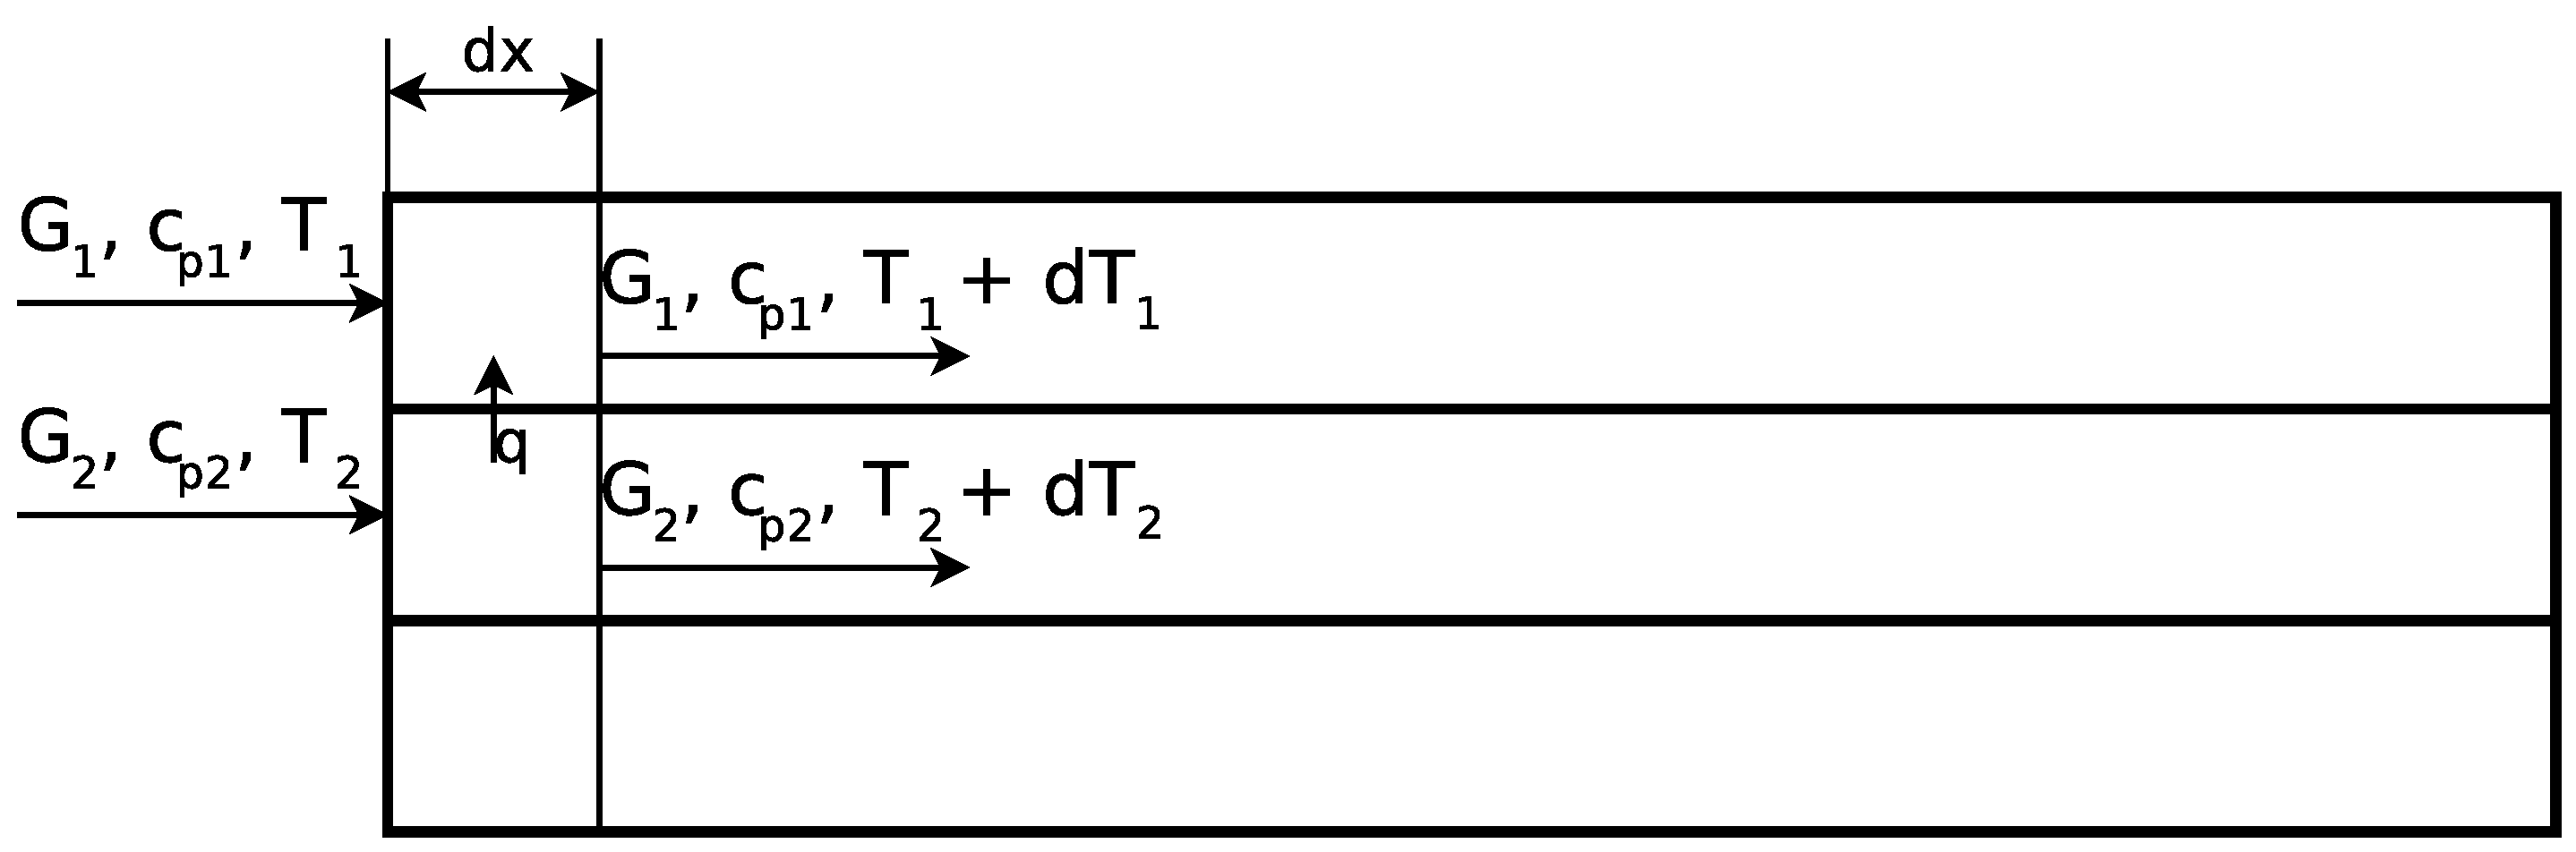
\includegraphics[width=\textwidth]{heat-scheme1.eps}
	\end{center}
	\caption{Схема потоков в прямоточном теплообменнике типа <<труба в трубе>>} \label{fig:heat.scheme1}
\end{figure}

Тепловой баланс холодного теплоносителя:
\begin{equation}\label{eq:tbal-cold}
	G_1 T_1 c_{p1}-G_1 c_{p1} (T_1+ d T_1) + q d F=0,
\end{equation}
где $G$ --- массовый расход, $c_p$ --- теплоемкость, $q$ --- тепловой поток, $F$ --- площадь поверхности теплообмена.

Поток тепла направлен от холодного теплоносителя к горячему, поэтому в выражении теплового баланса будет с отрицательным знаком:
\begin{equation}\label{eq:tbal-hot}
	G_2 T_2 c_{p2} -G_2 c_{p2} (T_2 + d T_2) - q d F =0.
\end{equation}

Поток тепла можно выразить уравнением теплопередачи:
\begin{equation}\label{eq:teploper}
	q=K(T_2-T_1),
\end{equation}
где $K$ --- коэффициент теплопередачи. Расписывая площадь поверхности теплопередачи через периметр сечения теплопередачи $P$ и длину элементарного объема $d x$ как $d F = d x P$, с использованием выражения \eqref{eq:teploper}, уравнения \eqref{eq:tbal-cold} и \eqref{eq:tbal-hot} можно переписать в виде системы:

 \begin{equation}
 \left\{
 \begin{aligned}
 &\dfrac{dT_1}{dx}=\dfrac{K(T_2-T_1)P}{G_1 c_{p1}}        \\
 &\dfrac{dT_2}{dx}=-\dfrac{K(T_2-T_1)P}{G_2 c_{p2}}            
 \end{aligned}
 \right.
 \end{equation}

В зависимости от поставленной задачи граничные условия могут задаваться по разному. Обычно известны расходы теплоносителей и температуры на входе теплообменника. Таким образом, в случае прямоточного теплообменника, для определения температур теплоносителя вдоль теплообменника решается задача Коши. 

Для противоточного теплообменника изменяется направление движения одного из теплоносителей. таки образом переписывая выражения тепловых балансов  можно записать следующую систему дифференциальных уравнений:
 \begin{equation}
 \left\{
 \begin{aligned}
 &\dfrac{dT_1}{dx}=\dfrac{K(T_2-T_1)P}{G_1 c_{p1}}        \\
 &\dfrac{dT_2}{dx}=\dfrac{K(T_2-T_1)P}{G_2 c_{p2}}            
 \end{aligned}
 \right. 
 \end{equation}
 
В случае противоточного теплообменника и известных входящих потоках необходимо решать краевую задачу.

Для плоской стенки коэффициент теплопередачи определяется как:
\begin{equation}
	K=\dfrac{1}{\dfrac{1}{\alpha_1} + \sum \dfrac{\delta}{\lambda} + \dfrac{1}{\alpha_2}},
\end{equation}
где $\alpha$ --- коэффициент теплоотдачи, $\delta$ --- толщина стенки, $\lambda$ --- коэффициент теплопроводности материала стенки, суммирование $\frac{\delta}{\lambda}$ проводится в случае если стенка состоит из нескольких слоев различного материала. 

Коэффициент теплоотдачи описывается критериальными уравнениями и зависит от многих факторов: конструкции аппарата, скорости движения жидкости физико-химических свойств и т.д. Обычно при решении задачи теплопередачи используются следующие критерии: Рейнольдса $Re=\dfrac{\bar{w} l \rho}{\mu}$, Прандтля $Pr=\dfrac{\mu c_p}{\lambda}$, Грасгофа $ Gr= g l^3 \beta_p \rho^2 \dfrac{\Delta T}{\mu^2}$, где $\bar{w}$ --- усредненная по сечению скорость движения теплоносителя, $l$ --- характерный размер аппарата, $\rho$ --- плотность теплоносителя, $\mu$ --- коэффициент вязкости, $c_p$ --- теплоемкость,  $\lambda$ --- теплопроводность, $g=9.8 м/с^2$, $\beta_p$ --- коэффициент объемного расширения, $\Delta T$ --- движущая сила теплоотдачи. При расчете коэффициентов теплоотдачи трубах в качестве характерного размера при определении критериев подобия выступает эквивалентный диаметр $D_э=\dfrac{4S}{P}$, где $S$ --- площадь сечения, $P$ --- периметр сечения.

Коэффициент теплоотдачи входит в выражение критерия Нуссельта: $Nu=\dfrac{\alpha l}{\lambda}$. Таким образом при определении коэффициентов теплоотдачи критериальное уравнение представляют в виде функции: $Nu= f (Re, Pr, Gr, ...)$
 
Ниже приведены выражения критерия Нуссельта для различных видов теплообменников и режимов течения \cite{pavlov}:
 \begin{itemize}
	 \item Теплоотдача в круглых трубах при турбулентном режиме ($Re>10000$):
		 \begin{equation}
		 	Nu=0.021 Re^{0.8} Pr^{0.43} \left( \dfrac{Pr}{Pr_{гр}} \right) ^{0.25} .
		 \end{equation}
	 \item Теплоотдача в круглых трубах при переходном режиме ($2300<Re<10000$):
		 \begin{equation}
		 	Nu=0.008 Re^{0.9} Pr^{0.43}.
		 \end{equation}
	 \item Теплоотдача в круглых трубах при ламинарном режиме течения:
		\begin{equation}
			Nu=0.17 Re^{0.33} Pr^{0.43} Gr^{0.1} \left( \dfrac{Pr}{Pr_{гр}} \right).
		\end{equation}
	 \item  Теплоотдача в кольцевом канале:
		 \begin{equation}
			  Nu=0.023 Re^{0.8} Pr^{0.4} \left(\dfrac{D_{вн}}{d_{н}}\right)^{0.45},
		 \end{equation}
		 где $D_{вн}$, $d_н$ --- внутренний и наружный  диаметр кольцевого сечения, характерным размером является $d_н$
	 \item Теплоотдача при перемешивании жидкостей мешалками:
	 \begin{equation}
		Nu=C Re^m Pr^{0.33} \left(\dfrac{\mu}{\mu_{ст}}\right)^{0.14}, \dfrac{\lambda}{D}
	 \end{equation}
	 где критерий Рейнольдса определяется как $Re=\frac{ \rho n d_m^2}{\mu}$, $D$ --- диаметр емкости, $n$ --- частота вращения мешалки, $\mu_{ст}$ --- динамический коэффициент вязкости жидкости при температуре стенки змеевика или рубашки, $\mu$ --- коэффициент вязкости при средней температуре жидкости, определяемой $(t_{ср.ж}+t_{ст})/2$. Для аппаратов с рубашками: $C=0.36$, $m=0.67$
\end{itemize}

Выражение для модели идеального смешения можно получить из теплового баланса всего теплообменника:
\begin{equation}
G_1 T_{1н} c_{p1}-G_1 c_{p1} T_1 + q F=0,
\end{equation}
где $T_{1н}$ --- температура на входе в теплообменник.
Данное выражение аналогично записи теплового баланса для элементарного объема теплообменника \eqref{eq:tbal-cold}. Подставляя выражение для теплового потока \eqref{eq:teploper} и преобразуя получим:
\begin{equation}
	T_1-T_{1н} = \dfrac{K(T_1-T_2)F}{G_1 c_{p1}}
\end{equation}

В случае, если температура второго теплоносителя изменяется по поверхности теплообменника, необходимо в качестве движущей силы использовать усредненную по поверхности разность температур: $\overline{(T_1-T_2)}=\dfrac{\int_{S} T_1 -T_2}{S}$

Вопросы для самоконтроля:
\begin{enumerate}
	\item Записать выражение теплового баланса теплообменника типа <<труба в трубе>> при наличии тепловых потерь.
	\item Как рассчитывается коэффициент теплопередачи?
	\item Как определяется коэффициент теплоотдачи?
\end{enumerate}

%В предлагаемых задачах можно считать теплофизические свойства не зависящими от температуры, следовательно в первом приближении  $\frac{Pr}{Pr_{ст}}=\frac{\mu}{\mu_{ст}}=1$, $\Delta T$ принять равным 5 С

